\documentclass[handout, t]{beamer}
\usepackage[latin1]{inputenc}
\usepackage{pgfpages}
\pgfpagesuselayout{2 on 1}[a4paper,border shrink=5mm]
\mode<handout>{\setbeamercolor{background canvas}{bg=black!5}}
\usecolortheme[named=BurntOrange]{}
\title[DIM3 Project Presentation]{CodeBuzz}
\author{Team Gocky}
\institute{University Of Glasgow}
\date{\today}
\begin{document}


\section{Aims}

\begin{frame}
\frametitle{CodeBuzz By Team Gocky}
Aims:
\begin{itemize}
\item Facilitate programming language learning by exposing beginners to
example programs written by industry experts and academics.
\item Aid reuse by providing a store of solutions to commonly recurring
problems.
\item Simple, usable, and clean user interface.
\end{itemize}
\end{frame}

\section{User Requirements}

\subsection{The Noob, The Experienced, and The Academic}

\begin{frame}
\frametitle{Barry The Noob}
Barry's programming ability is, at best,
amateur. He relies heavily on introductory texts and Internet forums
since his school does not provide learning materials for the language
of interest.
\begin{itemize}
\item Goals
    \begin{itemize}
    \item Finding code snippets to perform a specific programming task,
    e.g. reading from a file.
    \item Looking for code in a particular language.
    \item To download/copy the code snippet for integration into their
    program.
    \item Comment on a snippet to ask questions if understanding is low.
    \end{itemize}
\item Behaviours
    \begin{itemize}
    \item Curiosity towards others' code for inspiration for their own code
    development. Looking for ideas on, `How it's done', etcetera.
    \item Impatient regarding the `slowness' of their learning, wanting to
    get their application up and running as soon as possible. Quick and
    dirty.
    \end{itemize}
\end{itemize}
\end{frame}

\begin{frame}
\frametitle{Joe The Academic}
Joe is a University Professor teaching computing. He wishes to contribute
code to a publicly accessible forum for his research area and provide
a social code-sharing space for his students where class examples could
be hosted.
\begin{itemize}
\item Goals
    \begin{itemize}
    \item Look for crowd-sourced examples of how, or how not to, code a certain
    programming function for use in class.
    \item Use as a platform for student-submitted code that can be peer-reviewed.
    \item Wishes to aid the learning of students and others in their programming.
    \end{itemize}
\item Behaviours
    \begin{itemize}
    \item Comment/rate student-submitted code as part of the learning process.
    \item Submits high quality code for re-use and to contribute to the Open
    Source community.
    \item Gives low ratings and disapproving comments to incorrect,
    inefficient or ugly code snippets to discourage beginners.
    %from adopting poor techniques or bad programming habits.
    \end{itemize}
\end{itemize}
\end{frame}


% I think the wireframes should be printed separately.
%\begin{frame}
%\frametitle{Wireframes}
%This is the wireframes for the application:
%\begin{itemize}
%\item Logged in user
%\item Annonymous user
%\item Jane reviewing a snippet.
%\end{itemize}
%\end{frame}

\begin{frame}
\frametitle{Joe's Walkthrough}
\begin{enumerate}
\item Joe logs in using his user details.
\item Joe is presented with the home screen.
\item Joe selects the C programming language from the language drop-down
menu.
\item Joe proceeds to write his C code into the main window.
\item Joe selects the `Data Structures' category from the category
drop-down menu.
\item Joe is finished creating his code snippet and clicks the `Submit'
button.
\item Joe logs out.
\end{enumerate}
\end{frame}

\subsection{User Needs Matrix}

\begin{frame}
\frametitle{User Needs Matrix}
Our User Needs Matrix will go here!
\end{frame}

% You should have this on a separate piece of paper.
%\begin{frame}
%\frametitle{Joe's C Code Snippet}
%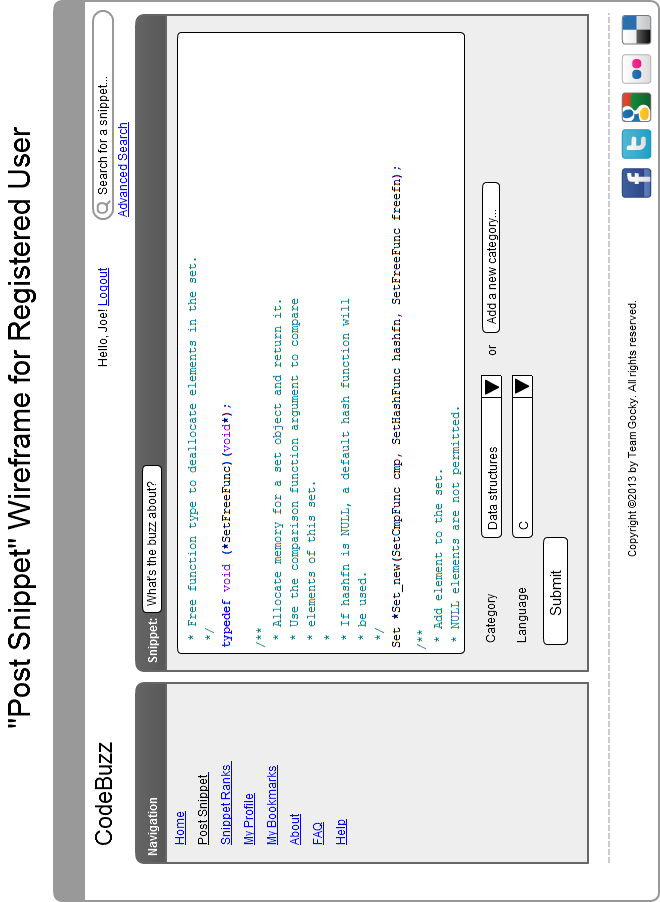
\includegraphics[width=\textwidth]{../imgs/CCodeSnippetHorz.png}
%\end{frame}

\end{document}
